\documentclass[10pt,twoside]{article}
\usepackage[utf8]{inputenc}
\usepackage{amsmath}
\usepackage{amsfonts}
\usepackage{amssymb}
\usepackage[spanish,es-noshorthands]{babel}
\usepackage[T1]{fontenc}
\usepackage{lmodern}
\usepackage{graphicx,hyperref}
\usepackage{tikz,pgf}
\usepackage{mathrsfs}
\usetikzlibrary{arrows}
\usepackage{multicol}
\usepackage{subfig}
\usepackage[papersize={6.5in,8.5in},includeheadfoot,left=0.4in,right=0.3in,top=0.3in,bottom=0.2in]{geometry}
\usepackage{fancyhdr}
\pagestyle{fancy}
\fancyhead[LE]{\url{http://gerdar.byethost9.com}}
\fancyhead[RE]{}
\fancyhead[RO]{\textit{Germ\'an Dar\'io Avenda\~no Ram\'irez, Lic - M.Sc.}}
\fancyhead[LO]{}

\author{Germ\'an Dar\'io Avenda\~no Ram\'irez, Lic. - M.Sc.}
\title{\begin{minipage}{0.15\textwidth}
\includegraphics[height=1.7cm]{Images/logo-colegio.png}
\end{minipage}\hfill \begin{minipage}{0.85\textwidth}\begin{center}
Prueba bimestral - ii período\\Cálculo y probabilidad$11^{\circ}$ -  formulario \textbf{1}\end{center}
\end{minipage}}
\date{}

\begin{document}
\maketitle
\section*{Cálculo}
\fbox{\emph{Responda las preguntas 1 a 3 de acuerdo con la siguiente información}}\\

El siguiente gráfico representa la posición respecto al tiempo de un cuerpo durante 12 segundos. El movimiento en tres intervalos de 4 segundos cada uno.

\begin{tikzpicture}[scale=0.8,yscale=0.5,xscale=0.8]
\draw[->] (0,0)node[left] {0} --(12.2,0) node[right]{$ t(s) $ };
\draw[<->] (0,-6.5) -- (0,8.5)node[left]{$ d(m) $};
\node[left]at(0,-6){-6};
\node[left]at(0,8){8};
\node[below] at (4,0){4};
\node[below] at (8,0){8};
\node[below] at (12,0){12};
\draw plot [domain=0:4] (\x, 2*\x);
\draw plot [domain=4:8] (\x,8);
\draw plot [domain=8:12](\x,-7/2*\x+36);
\draw[dashed](4,0)--(4,8);
\draw[dashed](8,0)--(8,8);
\draw[dashed](12,-6)--(12,0);
\draw[dashed](0,8)--(4,8);
\draw[dashed](0,-6)--(12,-6);
\end{tikzpicture}
\begin{enumerate}
  \item Respecto al movimiento realizado por el cuerpo en el intervalo de 4 a 8 segundos, podemos afirmar que
  \begin{enumerate}
    \item el cuerpo parte de la posición 4 y recorre con velocidad constante 8 metros.
    \item el cuerpo permanece en reposo, ya que mantiene la misma posición, mientras transcurren los 4 segundos.
    \item el cuerpo cambia la dirección del movimiento y recorre 4 metros más en una superficie plana.
    \item el cuerpo recorre 4 metros con velocidad constante en 8 segundos.
  \end{enumerate}
  \item Según la gráfica, se puede inferir que la velocidad del cuerpo en el transcurso de 8 a 12 segundos fue negativa, lo cual indica que
  \begin{enumerate}
    \item el cuerpo disminuyó la velocidad que venía manteniendo en el intervalo de 4 a 8 segundos.
    \item el cuerpo se devolvió seis metros más, desde el punto de partida.
    \item el cuerpo redujo el espacio recorrido durante los cuatro segundos respecto a los intervalos anteriores.
    \item el cuerpo recorrió la misma distancia, pero empleó más tiempo que en los intervalos anteriores.
  \end{enumerate}
  \item En el intervalo de 12 a 16 segundos se produjo un movimiento representado por la función: $ f(t)=\frac{3}{4}t-15 $. La interpretación de este movimiento realizado por el cuerpo es
  \begin{enumerate}
    \item el cuerpo recorrió tres metros durantes los cuatro segundos
    \item el cuerpo incrementó su velocidad en 5 metros por cada segundo
    \item el cuerpo retrocedió 15 metros durante el intervalo de tiempo.
    \item el cuerpo disminuyó su velocidad en dos metros durantes los cuatro segundos.
  \end{enumerate}
    \item Sean\\
  \textbf{P} la gráfica de la función $ y=x^2-2x+3 $\\
  \textbf{Q} la gráfica de la función $ y=x^2+2x+1 $\\
  Considere las siguientes afirmaciones suponiendo que \textbf{P} y \textbf{Q} están trazadas en el mismo sistema de coordenadas
  \begin{itemize}\begin{multicols}{2}
    \item[I] \textbf{P} y \textbf{Q} coinciden
    \item[II] \textbf{P} está a la izquierda de \textbf{Q}
    \item[III] \textbf{P} está a la derecha de \textbf{Q}
    \item[IV] \textbf{P} está más arriba que \textbf{Q}
    \item[V] \textbf{P} está más abajo que \textbf{Q}
  \end{multicols}
  \end{itemize}
      De las anteriores afirmaciones es o son verdaderas
    \begin{enumerate}\begin{multicols}{4}
      \item sólo I
      \item II y V
      \item II y IV
      \item III y IV      
    \end{multicols}
    \end{enumerate}
  \item Una compañía de taxis cobra una tarifa de \$3.000 por el primer kilómetro o fracción de kilómetro recorrida y \$1.000 por cada kilómetro o fracción adicional. ¿Cuál de las siguientes gráficas representa la relación entre el costo de un viaje $y$ y el número de kilómetros recorridos $x$?\\
\begin{minipage}{0.45\textwidth}
  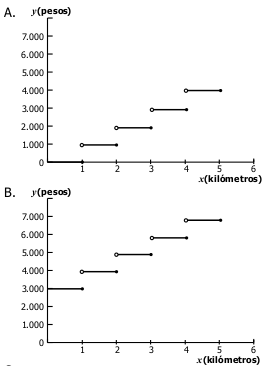
\includegraphics[scale=.65]{Images/grafica-taxi.png}
\end{minipage}\hfill
\begin{minipage}{.45\textwidth}
  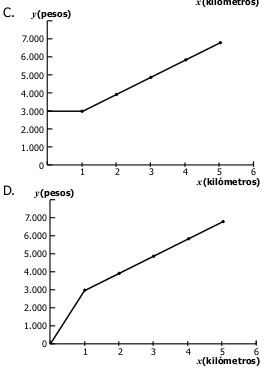
\includegraphics[scale=.65]{Images/grafica-taxi-2.png}
\end{minipage}
  \item Una recta que \textbf{no} intercepta al eje \textbf{x} en el punto $ x=2 $ tiene por ecuación
  \begin{enumerate}\begin{multicols}{2}
    \item $ x-2y=4 $
    \item $ 3x+y-6=0 $
    \item $ x-3y=2 $
    \item $ 5x-4y=10 $
  \end{multicols}
  \end{enumerate}
  \item Una raíz real de una función $ f $ es un número real $ r $ que satisface $ f(r)=0 $. Observando las siguientes gráficas, de las raíces de las funciones $ f$, $g $ y $ h $ se puede afirmar que
  \begin{minipage}{0.6\textwidth}
    \begin{enumerate}
    \item $ f $ y $ h $ tienen una raíz real en común
    \item $ g $ tiene cuatros raíces reales
    \item $ f $ y $ g $ tienen una raíz real en común
    \item $ h $ tiene una raíz real
  \end{enumerate}
  \end{minipage}\hfill
  \begin{minipage}{0.45\textwidth}
\definecolor{ffvvqq}{rgb}{0.44313725490196076,0.44313725490196076,0.44313725490196076}
\definecolor{qqqqff}{rgb}{0.3333333333333333,0.3333333333333333,0.3333333333333333}
\definecolor{qqwuqq}{rgb}{0.12941176470588237,0.12941176470588237,0.12941176470588237}
\begin{tikzpicture}[line cap=round,line join=round,>=triangle 45,x=1.0cm,y=1.0cm,scale=.5]
\draw[->,color=black] (-2.26,0.) -- (3.94,0.);
\draw[->,color=black] (0.,-3.14) -- (0.,5.2);
\clip(-2.26,-3.14) rectangle (3.94,5.2);
\draw[line width=1.2pt,color=qqwuqq,smooth,samples=100,domain=-2.260000000000001:3.939999999999996] plot(\x,{0-(\x)*((\x)-2.0)});
\draw[line width=1.2pt,color=qqqqff,smooth,samples=100,domain=-2.260000000000001:3.939999999999996] plot(\x,{(\x)*((\x)+1.0)*((\x)-1.0)});
\draw[line width=1.2pt,color=ffvvqq,smooth,samples=100,domain=-2.260000000000001:3.939999999999996] plot(\x,{((\x)-1.0)^(2.0)+1.0});
\begin{scriptsize}
\draw (-0.9,-2.06) node {$f$};
\draw (-1.6,-1.3) node {$g$};
\draw (-0.94,3.46) node {$h$};
\end{scriptsize}
\end{tikzpicture}
  \end{minipage}
  \item Se dice que una función $ f $ es creciente si $ f(x_1)<f(x_2) $ siempre que $ x_1<x_2 $ para números reales cualesquiera $ x_1 $ y $ x_2 $. Entre las siguientes gráficas, la que representa una función creciente es
  \begin{center}
  \begin{tikzpicture}
  \draw [<->](0,-1)node[below]{A}--(0,1);
  \draw [<->](-1,0)--(3,0)node[right]{$ x $};
  \draw plot [domain=-1:3](\x,{sin(\x r)});
  \draw [<->](5,-1)node[below]{B}--(5,1);
  \draw [<->](4,0)--(6,0);
  \draw plot [domain=4:6] (\x,{(-1/2)*\x+3});
  \draw [<->](7,0)--(9,0);
  \draw[<->](8,-1)node[below]{C}--(8,2);
  \draw plot [domain=7:9](\x,{exp(\x-8)});
  \draw [<->] (10,0)--(12,0);
  \draw[<->](11,-1)node[below]{D}--(11,1);
  \draw plot [domain=10:12](\x,{0.6});
  \end{tikzpicture}
  \end{center}
    \item Observe las gráficas de las funciones $ f $ y $ g $ que se presentan a continuación.
    
    \begin{minipage}{0.5\textwidth}
\definecolor{ttqqqq}{rgb}{0.2,0.,0.}
\definecolor{cqcqcq}{rgb}{0.7529411764705882,0.7529411764705882,0.7529411764705882}
\begin{tikzpicture}[line cap=round,line join=round,>=triangle 45,x=1.0cm,y=1.0cm,scale=.5]
\draw [color=cqcqcq,, xstep=1.0cm,ystep=1.0cm] (-5.16,-4.48) grid (5.32,4.1);
\draw[->,color=black] (-5.16,0.) -- (5.32,0.);
\foreach \x in {1}
\draw[shift={(\x,0)},color=black] (0pt,2pt) -- (0pt,-2pt) node[below] {\footnotesize $\x$};
\draw[->,color=black] (0.,-4.48) -- (0.,4.1);
\foreach \y in {1}
\draw[shift={(0,\y)},color=black] (2pt,0pt) -- (-2pt,0pt) node[left] {\footnotesize $\y$};
\draw[color=black] (0pt,-10pt) node[right] {\footnotesize $0$};
\clip(-5.16,-4.48) rectangle (5.32,4.1);
\draw[line width=1.2pt,smooth,samples=100,domain=-5.159999999999997:5.3199999999999985] plot(\x,{0-(3.0/16.0*(\x)^(2.0)+3.0/8.0*(\x)+51.0/16.0-6.0)});
\draw[line width=1.2pt,color=ttqqqq,smooth,samples=100,domain=-5.159999999999997:5.3199999999999985] plot(\x,{4.0/9.0*(\x)^(2.0)-4.0});
\begin{scriptsize}
\draw (-4.5,0.24) node {$f$};
\draw (-3.75,3.5) node {$g$};
\end{scriptsize}
\end{tikzpicture}
\end{minipage}\hfill
    \begin{minipage}{0.4\textwidth}
          De las siguientes afirmaciones
      \begin{itemize}
        \item[I] $ f(4)=g(4)=0 $
        \item[II] $ f $ y $ g $ tienen el mismo dominio
        \item[III] $ f(t)> g(t) $
        \item[IV] $ f $ y $ g $ interceptan el eje $ x $ en un único punto
        \item[V] $ g(x)> f(x) $ para todo $ x $ en el intervalo $ [-4,4] $
      \end{itemize}
      \end{minipage}
      
      Es o son verdaderas
      \begin{enumerate}\begin{multicols}{4}
        \item I y II
        \item II y IV
        \item solamente II
        \item solamente IV
      \end{multicols}
      \end{enumerate}
    \item Sea $ f(x)=\dfrac{x+2}{2x} $. Considere las siguientes afirmaciones:
    \begin{multicols}{2}
      \begin{itemize}
        \item[I] $ f(x)=0 $ sólo si $ x=-2 $
        \item[II] $ f(x+1)=f(x)+\frac{1}{2} $
        \item[III] $ f(3x)=3f(x) $
        \item[IV] Si $ f(x)=1 $, entonces $ x=2 $
      \end{itemize}
          \end{multicols}
      De las anteriores afirmaciones son  verdaderas
      \begin{multicols}{4}
        \begin{enumerate}
          \item I y III
          \item II y IV
          \item II y III
          \item I y IV
        \end{enumerate}
      \end{multicols}
      \end{enumerate}
\section*{Probabilidad}
\begin{enumerate}
  \item Al lanzar una vez un par de dados, la probabilidad de que salgan dos números consecutivos es:
\begin{multicols}{4}
  \begin{enumerate}
    \item $ \frac{10}{21} $
    \item $ \frac{5}{21} $
    \item $ \frac{10}{36} $
    \item $ \frac{5}{36} $
  \end{enumerate}
\end{multicols}
  \item En una bolsa se tienen 3 bolas rojas, 4 bolas blancas y 4 bolas azules. Se saca una bola al azar y ésta es de color azul. Si esta bola no se devuelve a la urna, ahora es más probable sacar al azar una bola \underline{\hspace{1.5cm}} que una bola \underline{\hspace{1.5cm}}
  \begin{multicols}{2}
\begin{enumerate}
    \item blanca - azul
    \item azul - blanca
    \item roja - azul
    \item azul - roja
    \end{enumerate}
  \end{multicols}
  \begin{minipage}{.4\textwidth}
      \item Si se lanza un caja de fósforos, ésta puede caer en cualquiera de las posiciones de la figura.
  \end{minipage}\hfill
  \begin{minipage}{.55\textwidth}
    \begin{center}
  
\includegraphics[scale=.55]{Images/fosforos.png}
  \end{center}
  \end{minipage}
  \begin{minipage}{.5\textwidth}
      \begin{center}
  \begin{tabular}{|c|c|}\hline
  \textbf{Posición}&\textbf{Probabilidad estimada}\\\hline
    1 & $ p(1)=0,65 $\\\hline
    2 & $ p(2)=0,22 $\\\hline
    3 & $ p(3)=0,13 $\\\hline
  \end{tabular}
  \end{center}
  \end{minipage}\hfill
  \begin{minipage}{.45\textwidth}
    La tabla construída después de efectuar 100 lanzamientos, muestra la probabilidad de caída en cada posición.
  \end{minipage}
  
  Después de otros cien lanzamientos más, se espera que
  \begin{enumerate}
    \item más de la mitad de las posiciones de caída corresponda a las posiciones 2 y 3
    \item las tres posiciones tengan aproximadamente la misma probabilidad entre ellas
    \item más de la mitad de todas las posiciones de caída corresponda a la posición 1
    \item el número de veces que cae la caja en la posición 2 se aproxime al 50\%
  \end{enumerate}
  \item  Un grupo de estudiantes construyó una ruleta. Después de jugar todo el día con ella y registrar los resultados, concluyó que la mayoría de las veces se detuvo en un número par y en pocas oca-
siones en una región sombreada.\\

¿Cuál fue la ruleta construída por los estudiantes?
\begin{center}
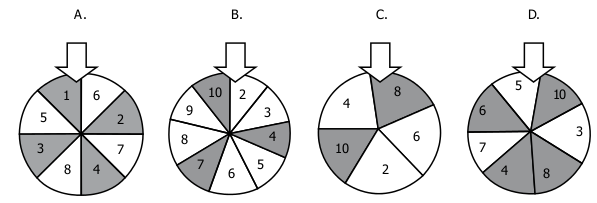
\includegraphics[scale=.55]{Images/ruletas.png}
\end{center}
\item En el noticiero de la noche anterior se anunció que había un 20\% de probabilidades de que lloviera y en realidad no llovió. Con relación a la afirmación del noticiero, usted diría no llovió porque:
\begin{enumerate}
  \item era uno de los sucesos posibles y era el que tenía mayor probabilidad. Habría error si se dijera que la probabilidad era del 100\% y no sucediera lo que se predecía.
\item es un error cuantificar la ocurrencia de un fenómeno del cual no se conocen todas las variables que lo determinan.
\item la probabilidad sólo mide la posibilidad de ocurrencia de un suceso, más no la certeza de su ocurrencia.
\item tal vez los que calcularon el dato se equivocaron o el periodista se equivocó y leyó un 20\% de probabilidades de que lloviera cuando era un 20\% de probabilidades de que no lloviera.
\end{enumerate}
\item Cuatro personas deciden jugar a los dados, para ello cada uno de los participantes debe elegir un dado de cuatro posibles. Gana quien en el lanzamiento obtenga mayor número
\begin{center}
\begin{tabular}{|c|p{1cm}|p{1cm}|p{1cm}|p{1cm}|p{1cm}|c|}\hline
  \textbf{Dados} & \multicolumn{6}{c|}{\textbf{Números que aparecen en las caras de los dados}}\\\hline
  A & 0 & 0 & 4 & 4 & 4 & 4\\\hline
  B & 3 & 3 & 3 & 3 & 3 & 3\\\hline
  C & 2 & 2 & 2 & 2 & 7 & 7\\\hline
  D & 1 & 1 & 1 & 5 & 5 & 5 \\\hline
\end{tabular}
\end{center}
Si se inicia la partida con un lanzamiento de las personas que eligieron el dado A y el dado B. La probabilidad de que el lanzamiento del dado A obtenga un número mayor al que obtiene el dado B es
\begin{enumerate}
  \item $ \frac{4}{2} $ ya que la probabilidad de que se pueda ganar con el dado A es la razón entre el número de aciertos y el número de fracasos o pérdidas
  \item $ \frac{2}{3} $ ya que el que tiene el dado B saca siempre 3, mientras quien tiene el dado A puede sacar 4, cuatro veces seis y con esto gana, o pierde si saca 0, que puede obtenerse dos veces seis.
  \item $ \frac{1}{3} $ ya que la probabilidad de que el dado A gane se establece como la diferencia entre la probabilidad de ganar del dado A menos la probabilidad del dado B, lo que es $ \frac{4}{6}-\frac{1}{3}=\frac{1}{3} $
  \item $ \frac{1}{2} $ ya que la probabilidad se obtiene haciendo el cociente entre lo obtenido en un dado y el total de los dados.
\end{enumerate}
\end{enumerate}
\newpage
\section*{Hoja de respuestas}
Formulario \textbf{1}\\

Nombre: \hrulefill Curso: \underline{\hspace{1cm}}  Fecha: \underline{\hspace{2cm}}\\
\begin{center}
\subsection*{Cálculo}
\begin{tabular}[scale=1.3]{|cccccccccc|}\hline
1 & 2 & 3 & 4 & 5 & 6 & 7 & 8 & 9 & 10\\
\textcircled{a} &\textcircled{a}&\textcircled{a}&\textcircled{a}&\textcircled{a} & \textcircled{a} & \textcircled{a}&\textcircled{a}&\textcircled{a}&\textcircled{a}\\
\textcircled{b}&\textcircled{b}&\textcircled{b}&\textcircled{b}&\textcircled{b} &\textcircled{b}&\textcircled{b}&\textcircled{b}&\textcircled{b}&\textcircled{b}\\
\textcircled{c}&\textcircled{c}&\textcircled{c}&\textcircled{c}&\textcircled{c}&\textcircled{c}&\textcircled{c}&\textcircled{c}&\textcircled{c}&\textcircled{c}\\
\textcircled{d}&\textcircled{d}&\textcircled{d}&\textcircled{d}&\textcircled{d}&\textcircled{d}&\textcircled{d}&\textcircled{d}&\textcircled{d}&\textcircled{d}\\\hline
\end{tabular}
\end{center}
\begin{center}
\subsection*{Probabilidad}
\begin{tabular}[scale=1.3]{|cccccc|}\hline
1 & 2 & 3 & 4 & 5 & 6\\
\textcircled{a}&\textcircled{a}&\textcircled{a}&\textcircled{a}&\textcircled{a}&\textcircled{a}\\
\textcircled{b}&\textcircled{b}&\textcircled{b}&\textcircled{b}&\textcircled{b}&\textcircled{b}\\
\textcircled{c}&\textcircled{c}&\textcircled{c}&\textcircled{c}&\textcircled{c}&\textcircled{c}\\
\textcircled{d}&\textcircled{d}&\textcircled{d}&\textcircled{d}&\textcircled{d}&\textcircled{d}\\\hline
\end{tabular}
\end{center}
\section*{Espacio para operaciones}
\newpage
\section*{Espacio para operaciones}
\end{document}
